% This is a Basic Assignment Paper but with like Code and stuff allowed in it, there is also url, hyperlinks from contents included. 

\documentclass[11pt]{article}

% Preamble

\usepackage[margin=1in]{geometry}
\usepackage{amsfonts, amsmath, amssymb}
\usepackage{fancyhdr, float, graphicx}
\usepackage[utf8]{inputenc} % Required for inputting international characters
\usepackage[T1]{fontenc} % Output font encoding for international characters
\usepackage{fouriernc} % Use the New Century Schoolbook font
\usepackage[nottoc, notlot, notlof]{tocbibind}
\usepackage{listings}
\usepackage{xcolor}
\usepackage{blindtext}
\usepackage{hyperref}
\hypersetup{
    colorlinks=true,
    linkcolor=black,
    filecolor=magenta,      
    urlcolor=cyan,
    pdfpagemode=FullScreen,
    }

\definecolor{codegreen}{rgb}{0,0.6,0}
\definecolor{codegray}{rgb}{0.5,0.5,0.5}
\definecolor{codepurple}{rgb}{0.58,0,0.82}
\definecolor{backcolour}{rgb}{0.95,0.95,0.92}

\lstdefinestyle{mystyle}{
    backgroundcolor=\color{backcolour},   
    commentstyle=\color{codegreen},
    keywordstyle=\color{magenta},
    numberstyle=\tiny\color{codegray},
    stringstyle=\color{codepurple},
    basicstyle=\ttfamily\footnotesize,
    breakatwhitespace=false,         
    breaklines=true,                 
    captionpos=b,                    
    keepspaces=true,                 
    numbers=left,                    
    numbersep=5pt,                  
    showspaces=false,                
    showstringspaces=false,
    showtabs=false,                  
    tabsize=2
}

\lstset{style=mystyle}

% Header and Footer
\pagestyle{fancy}
\fancyhead{}
\fancyfoot{}
\fancyhead[L]{\textit{\Large{Internet of Things Lab Assignment 2}}}
\fancyhead[R]{\textit{\Large{Krishnaraj}}}
\fancyfoot[C]{\thepage}
\renewcommand{\footrulewidth}{1pt}



% Other Doc Editing
% \parindent 0ex
%\renewcommand{\baselinestretch}{1.5}

\begin{document}

\begin{titlepage}
	\centering

	%---------------------------NAMES-------------------------------

	\huge\textsc{
		MIT World Peace University
	}\\

	\vspace{0.75\baselineskip} % space after Uni Name

	\LARGE{
		Internet of Things\\
		Second Year B. Tech, Semester 2
	}

	\vfill % space after Sub Name

	%--------------------------TITLE-------------------------------

	\rule{\textwidth}{1.6pt}\vspace*{-\baselineskip}\vspace*{2pt}
	\rule{\textwidth}{0.6pt}
	\vspace{0.75\baselineskip} % Whitespace above the title



	\huge{\textsc{
			Arudino with Sensors and Actuators
		}} \\



	\vspace{0.5\baselineskip} % Whitespace below the title
	\rule{\textwidth}{0.6pt}\vspace*{-\baselineskip}\vspace*{2.8pt}
	\rule{\textwidth}{1.6pt}

	\vspace{1\baselineskip} % Whitespace after the title block

	%--------------------------SUBTITLE --------------------------	

	\LARGE\textsc{
		Assignment 2
	} % Subtitle or further description
	\vfill

	%--------------------------AUTHOR-------------------------------

	Prepared By
	\vspace{0.5\baselineskip} % Whitespace before the editors

	\Large{
		Krishnaraj Thadesar \\
		Cyber Security and Forensics\\
		Batch A2, PA 20
	}


	\vspace{0.5\baselineskip} % Whitespace below the editor list
	\today

\end{titlepage}


\tableofcontents
\thispagestyle{empty}
\clearpage

\setcounter{page}{1}

\section{Aim}
To interface following Sensors such as Temperature or Ultrasonic or IR or any other sensor with Arduino Uno and display the output on the Serial Monitor.
\section{Objectives}
\begin{itemize}
	\item To interface Temperature Sensor with Arduino Uno and display the output on the Serial Monitor.
	\item To learn how to use Arduino Uno.
	\item To learn about Actuators and Sensors.
\end{itemize}
\section{Equipments Required}
\begin{table}[H]
	\begin{tabular}{|c|c|c|}
		\hline
		\textbf{Name} & \textbf{Quantity} & \textbf{Component}             \\ \hline
		U1            & 1                 & Arduino Uno R3                 \\ \hline
		U5            & 1                 & Temperature Sensor {[}TMP36{]} \\ \hline
		PIEZO1        & 1                 & Piezo                          \\ \hline
		D1            & 1                 & Red LED                        \\ \hline
		MFAN          & 1                 & DC Motor                       \\ \hline
		R1            & 1                 & 1 kΩ Resistor                  \\ \hline
	\end{tabular}
\end{table}

\section{Theory}
In this assignment, we will be interfacing a temperature sensor with Arduino Uno and displaying the output on the serial monitor. The temperature sensor used in this project is an analog sensor, which measures temperature by outputting a voltage proportional to the temperature. The TMP36 temperature sensor is a popular choice due to its accuracy and low cost.\\

The Arduino Uno is a microcontroller board that is commonly used for prototyping and educational purposes. It has 14 digital input/output pins and 6 analog input pins, and is powered by a 5V supply. The board is programmed using the Arduino programming language, which is a simplified version of C++.\\

To interface the temperature sensor with the Arduino, we connect the output pin of the sensor to one of the analog input pins on the Arduino, and connect the ground and power pins to the appropriate pins on the Arduino. We then read the analog voltage from the sensor using the analogRead() function in the Arduino code.\\

The output of the temperature sensor is displayed on the serial monitor, which is a useful tool for debugging and monitoring the output of the Arduino. The serial monitor allows us to view the output in real-time and make any necessary adjustments to the code or hardware.\\

In the context of the Internet of Things (IoT), this project can be extended to include wireless communication, allowing the temperature readings to be monitored and analyzed remotely. For example, the Arduino could be connected to a Wi-Fi module or a cellular module, and the temperature readings could be sent to a cloud-based platform for analysis and visualization. This could be useful in applications such as environmental monitoring or industrial automation.


\section{Platform}
\textbf{Operating System}: Arch Linux x86-64 \\
\textbf{IDEs or Text Editors Used}: Arduino IDE\\
\textbf{Compilers} : g++ and gcc on linux for C++\\

\section{Circuit}
\begin{figure}[H]
	\centering
	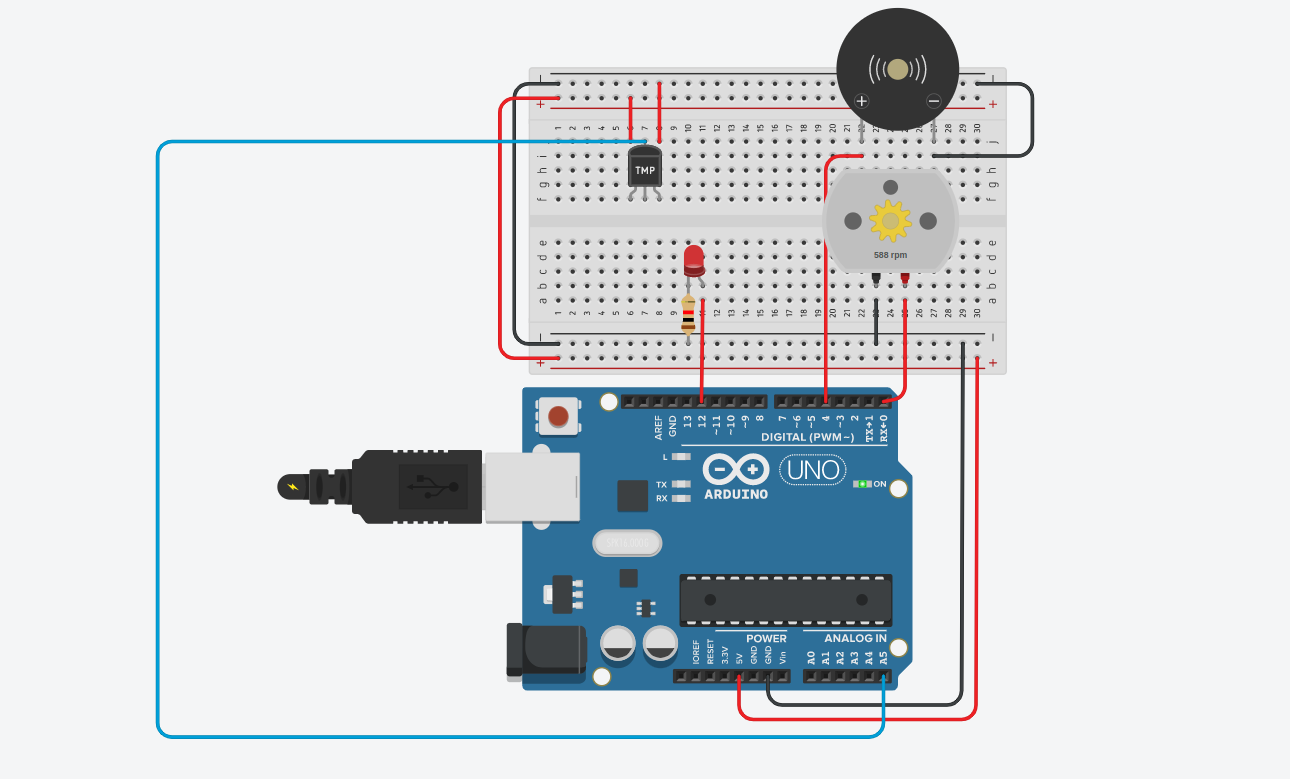
\includegraphics[width=.95\textwidth]{Screenshot_on_2023-05-02_at_00-05-46.png}
	\caption{Tinkercad Circuit}
\end{figure}

\section{Circuit Diagram}

\begin{figure}[H]
	\centering
	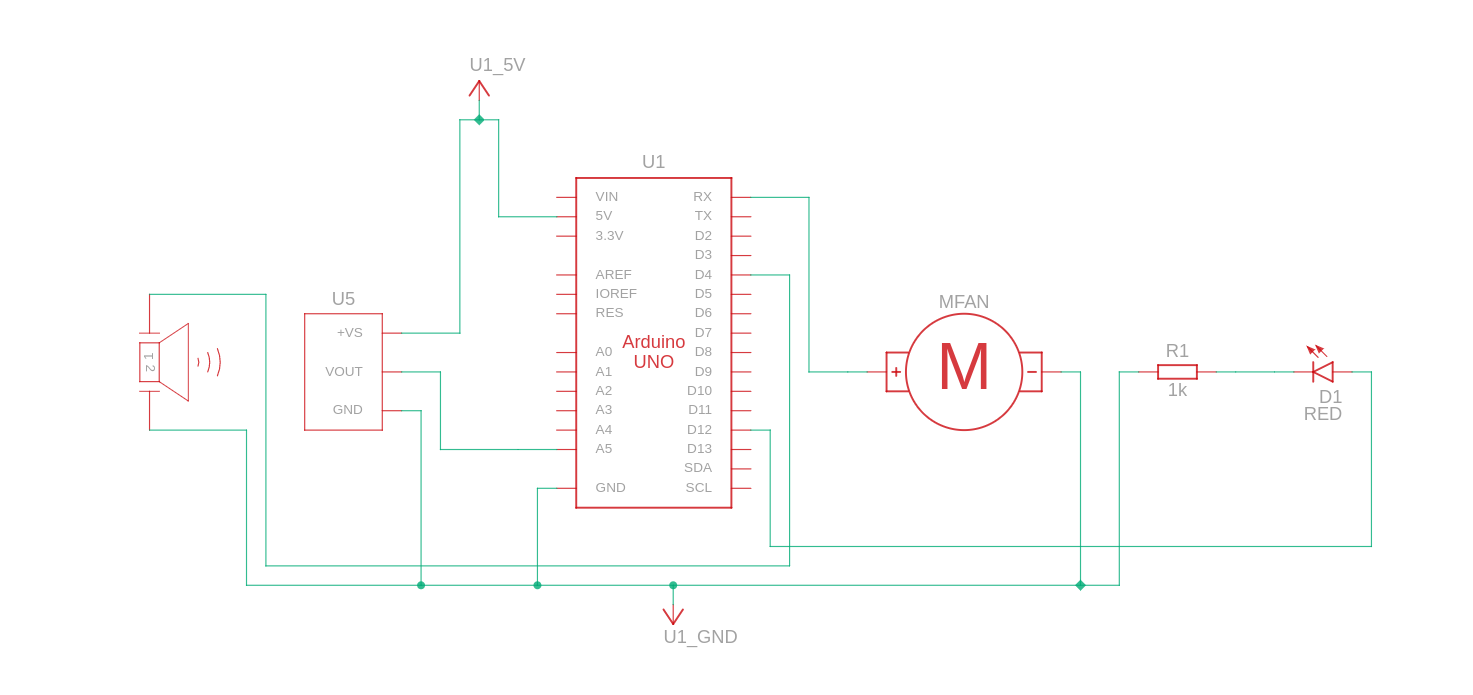
\includegraphics[width=.95\textwidth]{Screenshot_on_2023-05-02_at_00-10-00.png}
	\caption{Circuit Diagram}
\end{figure}

\section{Input}
Input from the Temperature Sensor TMP36
\section{Output}
\begin{verbatim}
Temperature is too much
153
Temperature is too much
153
27
27
20
20
\end{verbatim}
\section{Code}
\begin{lstlisting}[language=C++]

#define LED_PIN 12
#define MOTOR_PIN 0
#define BUZZER_PIN 4
int analogPin = A5; 
int val = 0; 


void setup() {
	Serial.begin(9600);  //  setup serial
	pinMode(LED_PIN, OUTPUT);
	pinMode(MOTOR_PIN, OUTPUT);
	pinMode(BUZZER_PIN, OUTPUT);
}

void loop() {
	val = analogRead(analogPin);  // read the input pin
	Serial.println(val); // debug value
	
	if(val > 100){
		Serial.println("Temperature is too much");
	digitalWrite(0, HIGH);
		digitalWrite(LED_PIN, HIGH);
	tone(BUZZER_PIN, val, 1000);
	}
}
\end{lstlisting}
\section{Conclusion}
Thus, we have successfully interfaced Temperature Sensor with Arduino Uno and displayed the output on the Serial Monitor.
\clearpage

\section{FAQ}
\begin{enumerate}
	\item Arduino Uno R3 (Code: U1)
	      \begin{itemize}
		      \item Type: Microcontroller board
		      \item Digital pins: 14
		      \item Analog input pins: 6
		      \item Operating voltage: 5V
		      \item Input voltage (recommended): 7-12V
		      \item Input voltage (limits): 6-20V
		      \item Flash memory: 32 KB (ATmega328P microcontroller)
		      \item SRAM: 2 KB (ATmega328P microcontroller)
		      \item EEPROM: 1 KB (ATmega328P microcontroller)
		      \item Clock speed: 16 MHz (ATmega328P microcontroller)
	      \end{itemize}
	\item Temperature Sensor [TMP36] (Code: U2)
	      \begin{itemize}
		      \item Type: Analog sensor
		      \item Pin 1: Output voltage (analog)
		      \item Pin 2: Ground
		      \item Pin 3: Input voltage (3.3V - 5V)
		      \item Temperature range: -40°C to +125°C
		      \item Output voltage range: 0V to 1.75V (at 25°C)

	      \end{itemize}
	\item  Buzzer (Code: U4)
	      \begin{itemize}
		      \item Type: Electromechanical transducer
		      \item Operating voltage: 5V to 12V
		      \item Sound frequency: 2kHz to 4kHz
		      \item Sound pressure level: 80dB to 110dB
		      \item Pin 1: Positive terminal (+)
		      \item Pin 2: Negative terminal (-)
	      \end{itemize}
	\item DC Motor:
	      \begin{itemize}
		      \item Type: Electromechanical motor
		      \item Operating voltage: Varies depending on the motor specifications, typically 3-12V
		      \item Maximum voltage: Varies depending on the motor specifications, typically 6-24V
		      \item Maximum current: Varies depending on the motor specifications, typically 100mA - 1A
		      \item Control type: Typically controlled using pulse width modulation (PWM)
		      \item Speed range: Varies depending on the motor specifications, typically 1000-5000 RPM
		      \item Direction of rotation: Can be reversed by reversing the polarity of the power supply
		      \item Shaft diameter: Varies depending on the motor specifications, typically 2-5mm
		      \item Stall torque: Varies depending on the motor specifications, typically 0.1-1 Nm
		      \item Gearbox: Some DC motors come with a gearbox for increased torque or reduced spee
	      \end{itemize}
\end{enumerate}


\end{document}